%==============================================================================
% queues-performance.tex
%==============================================================================

\chapter{Performance}
\label{chap:queues-performance}

We evaluate the performance of the different queue implementations
with a variety of parallel Java Grande Forum benchmarks (Appendix
\ref{chap:appendix-benchmarks}) on two different machines:

\begin{itemize}
\item Intel Core2 Duo with one processor and two cores, running Ubuntu
  10.04 64-bit with kernel 2.6.32 and Sun Hotspot JDK 1.6.0\_20
  (Appendix \ref{sec:experimental-setup-marvin})
\item Intel Nehalem with two processors and eight cores, running
  Ubuntu 9.04 64-bit with kernel 2.6.29 and Sun Hotspot JDK 1.6.0\_20
  (Appendix \ref{sec:experimental-setup-mafushi})
\end{itemize}

Both machines invoke the JVM with the following parameters:

\begin{lstlisting}
  -server -Xmx2048M -Xms2048M -Xss8m
\end{lstlisting}

The execution time reported is the average of the three best benchmark
iterations from ten separate invocations.

\begin{figure}[ht]
  \centering
  \subfigure[Intel Core2 Duo: 2 threads, 2 workers]{
    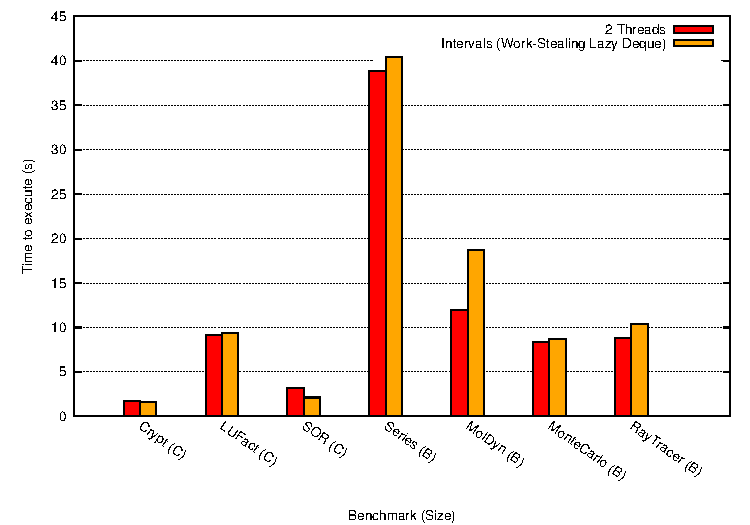
\includegraphics[width=0.47\linewidth]{queues-evaluation/marvin-threads}
    \label{fig:queues-evaluation-marvin-threads}
  }
  \subfigure[Intel Nehalem: 8 threads, 8 workers]{
    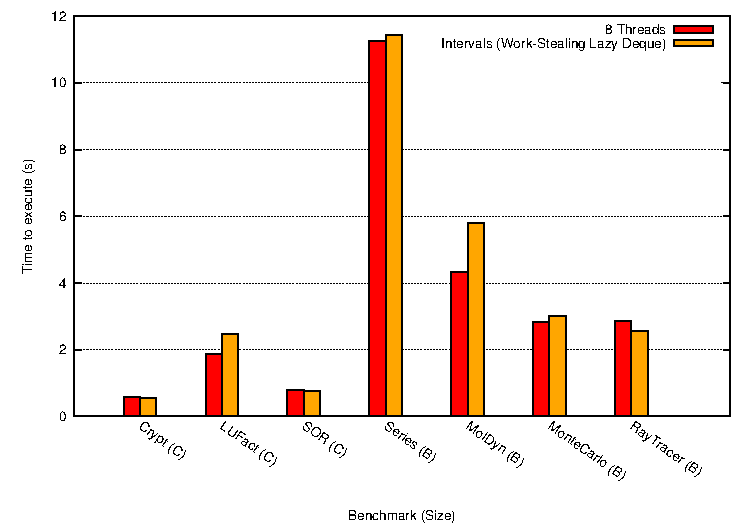
\includegraphics[width=0.47\linewidth]{queues-evaluation/mafushi-threads}
    \label{fig:queues-evaluation-mafushi-threads}
  }
  \caption{Threads and intervals benchmarks running on Intel Core2 Duo
    (Appendix \ref{sec:experimental-setup-marvin}) and Intel
    Nehalem (Appendix \ref{sec:experimental-setup-mafushi})}
  \label{fig:queues-evaluation-threads}
\end{figure}

\todo[inline]{Finish chapter \emph{Performance}}

\begin{itemize}
\item Benchmarks
\item Idempotent FIFO and LIFO queue, deque; duplicating queues
\item Global shared work queue
\item $\le 8$ cores
\end{itemize}

To validate the design of intervals, we are in the process of porting
a number of threaded benchmarks to use intervals, beginning with the
Java Grande Forum's multithreaded benchmarks. The benchmarks we have
ported so far make use of the many of the patterns presented in this
paper, including point-to-point synchronization (SOR), barriers
(MolDyn), and fork-join sections (Crypt, LUFact, Series, MonteCarlo,
and RayTracer). We have found that using intervals results in fewer
lines of code when compared against the original threaded
versions. Performance generally improves as well due to the improved
load balancing offered by a work-stealing execution engine.

\section{References}

\subsection{Dynamic circular work-stealing deque \cite{Chase2005}}

We evaluated the performance of the new dynamic circular work-stealing
algorithm in comparison to the original fixed-array ABP work-stealing
algorithm. We implemented both algorithms in C++, and used a simple
shared pool algorithm that allocates and frees a buffer with a single
CAS instruction.

The benchmark we ran simulates load balancing of a general computation
by building the DAG corresponding to the computation
\cite{Blumofe1999}, as follows: Initially a single deque contains a
single node representing the first work item of the
computation. Processes pop nodes from their own deques, and
\lstinline!steal! nodes from other deques if their own deque is
empty. Each time a process pops a node from a deque, it generates up
to B child nodes, and pushes them into its deque (B represents the
maximum branch of the DAG, and it is a configurable parameter). The
number of child nodes generated for a node is randomly chosen with
probability that is inversely proportional to the depth of that node
in the DAG. The expected number of child nodes for a node of depth $d$
in a DAG of maximum depth $D$ is: $B \cdot \left(1 - \frac{d}{D}
\right)$. To get the most accurate measure of the performance
difference between the two algorithms, we did not perform any work on
a node other than pushing its child nodes to the process's deque.

We ran the benchmark on a 16 node Sun Enterprise 6500, an SMP machine
formed from 8 boards of two 400MHz UltraSparc processors, connected by
a crossbar UPA switch, and running a SolarisTM 9 operating system. We
chose the maximum branch of the DAG to be 13, and the maximum depth to
be 10. We used 72-element arrays for the original ABP deques, and our
algorithm allocated the deques with an initial size of 64-elements,
plus a few 128-element arrays in the shared pool.

Figure 9 presents the throughput of both algorithms, running
stand-alone, as a function of the number of processes. As can be
seen, both algorithms scale well, and the performance difference is
relatively small. Recall that our benchmark does not perform any real
computation -- it only measures the load-balancing algorithm
overhead. In real applications the time spent on the load-balancing
algorithm Next we ran our benchmark in a multiprogrammed fashion by
running multiple instances of it in parallel, where each instance is
running with 16 processes (as the number of processors on the
machine). Figure 10 presents the throughput of an instance as a
function the multiprogramming level. As can be seen, there is no
significant difference in the performance of the two algorithms.

To compare the stability of the two algorithms, we measured how many
of our 64-element arrays overflowed and needed a 128-element array
from the shared pool, and noticed that at most one 128-element array
is ever needed. On the other hand, the 72-element array allocated for
each of the deques in the original ABP algorithm was not always
sufficient, and in some cases the algorithm failed to complete due to
an overflow of an array. These failures became more frequent as the
level of multiprogramming increased. Therefore, for the same amount of
array space (notice that $16 \cdot 72 = 128 + (16 \cdot 64)$), we get
more robustness with our new algorithm than with the original ABP
algorithm, without a noticeable cost in performance.

\subsection{Avoid \lstinline!top! accesses in \lstinline!put()!}

Unlike the original ABP algorithm, the new algorithm requires reading
\lstinline!top! on every execution of the \lstinline!put()!
operation. This may result in more data-cache misses compared to the
original algorithm (recall that unlike \lstinline!bottom!,
\lstinline!top! is modified by all processes).

The frequency of accesses to the \lstinline!top! variable can be
significantly reduced, by keeping a local upper bound on the size of
the deque, and only read \lstinline!top! when the upper bound
indicates that an array expansion may be necessary. Such a local upper
bound can be easily achieved by saving the last value of
\lstinline!top! read in a local variable, and using this variable to
compute the size of the deque (instead of the real value of
\lstinline!top!). Because \lstinline!top! is never decremented, the
real size of the deque can only be smaller than the one calculated
using this local variable.

\minisec{Herlihy}

The ability to resize carries a price: every call must read
\lstinline!top! (Line 21) to determine if a resize is necessary,
possibly causing more cache misses because \lstinline!top!  is
modified by all processes. We can reduce this overhead by having
threads save a local value of \lstinline!top!  and using it to compute
the size of the \lstinline!UnboundedDEQueue!  object. A thread reads
the \lstinline!top!field only when this bound is exceeded, indicating
that a \lstinline!resize()! may be necessary.  Even though the local
copy may become outdated because of changes to the shared
\lstinline!top!, \lstinline!top! is never decremented, so the real
size of the \lstinline!UnboundedDEQueue! object can only be smaller
than the one calculated using the local variable.

\subsection{Work-Stealing}

Chapter \ref{chap:queues-background} summarizes the properties of
work-stealing queues and introduces ``lazy deque'', the queue
currently used by the intervals scheduler. Chapter
\ref{chap:queues-implementation} describes the investigated queue
implementations. None of the approaches that were developed as part of
this research yielded a queue that was improving work-stealing
performance on the machines we had to test them with (Appendix
\ref{sec:experimental-setup-marvin} and
\ref{sec:experimental-setup-mafushi}). Possible reasons for this are
given in the performance evaluation in Chapter
\ref{chap:queues-performance}. Chapter\ref{chap:queues-conclusions}
concludes and summarizes the encountered problems in order to preserve
this research for future reference.


%%% Local Variables: 
%%% mode: latex
%%% TeX-master: "thesis"
%%% End: 
